\part{Discos}

\begin{figure}[h!]
    \centering
    \includegraphics[width=0.6\textwidth]{imgs/disk_types.jpg}
    \caption{Tipos de discos de armazenamento.}
\end{figure}

% ------------------------------------------------------------------------
\chapter{Processo de Boot}\label{chap:boot}
% ------------------------------------------------------------------------
O processo de inicialização (\textit{boot}) é a sequência de operações que o computador realiza ao ser ligado para carregar o sistema operacional. O termo deriva de "pull oneself up by one’s bootstraps". Conceitos fundamentais de boot e interação com o kernel são discutidos em \cite{tanenbaum:mos,silberschatz:osc,love:linuxkernel}.

\section{BIOS e ROM}\label{sec:bios}
O processo inicia-se na ROM (\textit{Read-Only Memory}), onde reside o BIOS (\textit{Basic Input/Output System}). O BIOS é gravado em um chip e é responsável pelo teste de hardware (POST) e pela inicialização básica. As configurações do BIOS (sequência de boot, data/hora) são armazenadas em uma memória CMOS alimentada por bateria.
Historicamente, evoluímos de memórias PROM (programáveis uma vez), EPROM (apagáveis por UV), EEPROM (apagáveis eletricamente) até as modernas Flash ROM, que permitem atualizações de firmware \cite{patterson:hennessy}. A padronização moderna de firmware segue a especificação \cite{uefi:spec}.

\section{UEFI e Legacy}\label{sec:uefi}
Nos anos 90, a Intel iniciou a substituição do BIOS pelo EFI, que evoluiu para o padrão UEFI (\textit{Unified Extensible Firmware Interface}) \cite{uefi:spec}.
\begin{itemize}
    \item \textbf{Legacy BIOS:} Utiliza o MBR para boot. Carrega apenas o primeiro estágio do \textit{bootloader} nos primeiros 446 bytes do disco.
    \item \textbf{UEFI:} Armazena na NVRAM o caminho para os carregadores. Utiliza uma partição específica (Partição EFI ou ESP), formatada geralmente em FAT32, onde residem os arquivos \texttt{.efi} dos sistemas operacionais.
\end{itemize}

\section{Gerenciadores de Boot}\label{sec:bootloaders}
O carregador de inicialização (\textit{bootloader}), como o GRUB ou LILO, é carregado pelo firmware. Sua função é carregar o Kernel do sistema operacional na memória RAM e transferir o controle para ele \cite{love:linuxkernel}. No Linux, o Kernel geralmente utiliza um sistema de arquivos temporário (\textit{initramfs}) para montar a partição raiz.

% ------------------------------------------------------------------------
\chapter{Memória Secundária}\label{chap:memoria-secundaria}
% ------------------------------------------------------------------------
A memória secundária, ou memória de massa, é não-volátil e utilizada para armazenar grandes quantidades de dados fora do processador \cite{patterson:hennessy}.

\section{Discos Rígidos (HDD)}\label{sec:hdd}
Dominaram o mercado por décadas. São compostos por discos magnéticos (pratos) e cabeças de leitura/gravação mecânicas.
\begin{itemize}
    \item \textbf{Geometria:} Organizados em Trilhas (círculos concêntricos), Setores (fatias das trilhas, geralmente 512 bytes) e Cilindros (conjunto de trilhas alinhadas verticalmente).
    \item \textbf{Endereçamento:} Antigamente usava-se CHS (Cylinder-Head-Sector). Modernamente utiliza-se LBA (\textit{Logical Block Addressing}), que trata o disco como uma sequência linear de blocos.
\end{itemize}

\section{Unidades de Estado Sólido (SSD)}\label{sec:ssd}
Utilizam memória Flash (NAND ou NOR), baseada em transistores que armazenam carga elétrica (bits) sem partes móveis \cite{nvme:spec}.
\begin{itemize}
    \item \textbf{Vantagens:} Alta velocidade de acesso, resistência a impactos e menor consumo de energia.
    \item \textbf{Estrutura:} Não possuem trilhas ou setores físicos, organizando-se em páginas e blocos. O protocolo NVMe (\textit{Non-Volatile Memory Express}) foi criado para explorar a velocidade do barramento PCIe, superando as limitações do padrão SATA.
\end{itemize}

\begin{figure}[h!]
    \centering
    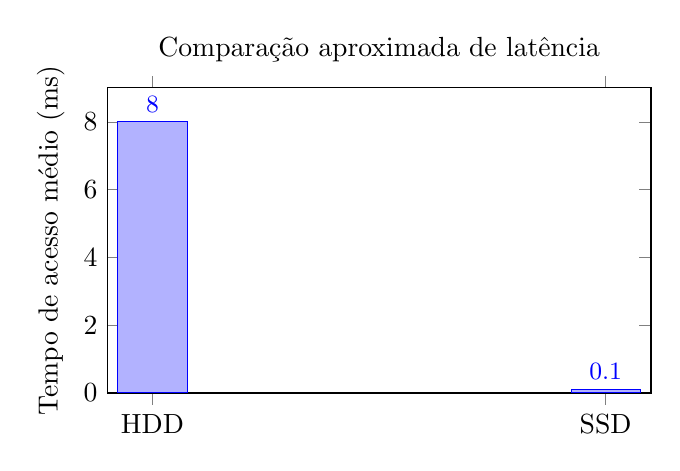
\begin{tikzpicture}
        \begin{axis}[
            ybar,
            width=0.7\textwidth,
            height=0.45\textwidth,
            bar width=25pt,
            ylabel={Tempo de acesso médio (ms)},
            symbolic x coords={HDD,SSD},
            xtick=data,
            ymin=0,
            ymax=9,
            nodes near coords,
            every node near coord/.append style={font=\small},
            title={Comparação aproximada de latência}
        ]
            \addplot coordinates {(HDD,8) (SSD,0.1)};
        \end{axis}
    \end{tikzpicture}
    \caption{Latência típica: HDD \textasciitilde8 ms vs SSD \textasciitilde0.1 ms.}\label{fig:latencia-hdd-ssd}
\end{figure}

\noindent A redução drástica de latência em SSDs impacta também estratégias de paginação discutidas no Capítulo \ref{chap:memoria}.

% ------------------------------------------------------------------------
\chapter{Partições}\label{chap:particoes}

\begin{figure}[h!]
    \centering
    \includegraphics[width=0.8\textwidth]{imgs/disk_partition.png}
    \caption{Particionamento de disco rígido.}
\end{figure}
% ------------------------------------------------------------------------
O particionamento divide o disco físico em unidades lógicas. Existem dois esquemas principais de tabelas de partição.

\section{MBR (Master Boot Record)}\label{sec:mbr}
O MBR localiza-se no primeiro setor do disco (512 bytes) \cite{gpt:efi}.
\begin{itemize}
    \item \textbf{Estrutura:} Contém a área de boot (446 bytes), a tabela de partições (64 bytes) e a assinatura (2 bytes).
    \item \textbf{Limitações:} Suporta apenas 4 partições primárias. Para contornar isso, criou-se a \textit{Partição Estendida}, que pode conter múltiplas \textit{Partições Lógicas}. Endereça no máximo 2TB de espaço devido ao limite de 32 bits.
\end{itemize}

\section{GPT (GUID Partition Table)}\label{sec:gpt}
Introduzido com o UEFI para superar as limitações do MBR (ver Seção \ref{sec:mbr}) \cite{gpt:efi,uefi:spec}.
\begin{itemize}
    \item \textbf{Características:} Utiliza endereçamento de 64 bits (suporta até 9.4 ZB). Permite um número praticamente ilimitado de partições (padrão de 128 no Windows).
    \item \textbf{Segurança:} Possui backup da tabela de partições no final do disco e CRC32 para verificação de integridade.
\end{itemize}


\begin{figure}[h!]
    \centering
    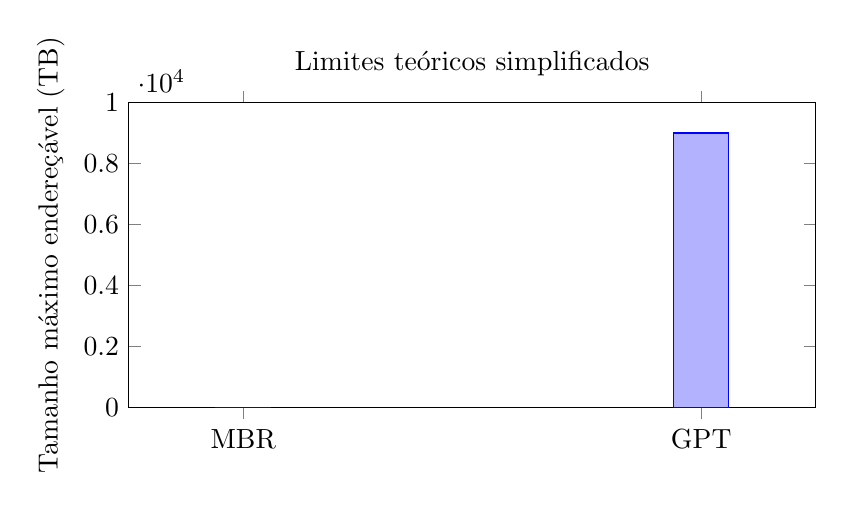
\begin{tikzpicture}
        \begin{axis}[
            ybar,
            width=0.85\textwidth,
            height=0.45\textwidth,
            bar width=20pt,
            ylabel={Tamanho máximo endereçável (TB)},
            symbolic x coords={MBR,GPT},
            xtick=data,
            ymin=0,
            ymax=10000,
            enlarge x limits=0.25,
            yticklabel style={/pgf/number format/fixed},
            title={Limites teóricos simplificados}
        ]
            % MBR ~2 TB, GPT muito maior (representamos 9000 TB como aproximação simbólica)
            \addplot coordinates {(MBR,2) (GPT,9000)};
        \end{axis}
    \end{tikzpicture}
    \caption{Diferença de capacidade entre MBR e GPT (valores ilustrativos).}\label{fig:capacidade-mbr-gpt}
\end{figure}

\noindent A maior capacidade e redundância da GPT cooperam com recursos avançados de sistemas de arquivos modernos (Capítulo \ref{chap:filesystem}).

\section{Gerenciamento}
Ferramentas como \texttt{fdisk}, \texttt{gdisk} e \texttt{parted} são usadas para criar partições. O comando \texttt{lsblk} lista dispositivos de bloco. Para uso, as partições devem ser formatadas e montadas (\texttt{mount}) em um diretório do sistema. O arquivo \texttt{/etc/fstab} controla as montagens automáticas no boot.

% ------------------------------------------------------------------------
\chapter{Sistema de Arquivos}\label{chap:filesystem}
% ------------------------------------------------------------------------
O Sistema de Arquivos (\textit{Filesystem}) é a estrutura lógica usada para organizar e armazenar dados nas partições. No Linux, o VFS (\textit{Virtual Filesystem}) abstrai os diferentes tipos de sistemas para o Kernel \cite{love:linuxkernel,tanenbaum:mos}.

\section{Conceitos Básicos}
\begin{itemize}
    \item \textbf{Área de Controle vs. Dados:} Metadados (permissões, datas, localização) ficam na área de controle; o conteúdo real fica na área de dados.
    \item \textbf{Inode (Index Node):} Estrutura fundamental no Linux que armazena os metadados de um arquivo. Cada arquivo é identificado por um número de inode único na partição.
    \item \textbf{Blocos:} Unidade mínima de alocação (geralmente 4KB).
\end{itemize}

\section{Famílias de Sistemas de Arquivos}
\begin{itemize}
    \item \textbf{Ext (Ext2, Ext3, Ext4):} Padrão no Linux. O Ext3 introduziu o \textit{journaling} \cite{tweedie:ext3}. O Ext4 suporta volumes de até 1 EB.
    \item \textbf{FAT (FAT16, FAT32, exFAT):} Comuns em pendrives e compatibilidade com Windows. Não suportam permissões POSIX nativamente e sofrem com fragmentação.
    \item \textbf{NTFS:} Padrão do Windows, suporta ACLs, compressão e \textit{journaling}.
    \item \textbf{Sistemas Modernos (CoW):} BtrFS \cite{rodeh:btrfs} e ZFS \cite{bonwick:zfs} utilizam \textit{Copy-on-Write}, snapshots e alta integridade; LFS \cite{rosenblum:lfs} explora escrita sequencial.
\end{itemize}

\begin{table}[h!]
    \centering
    \begin{adjustbox}{width=\textwidth}
        \centering
        \begin{tabular}{|l|c|c|c|c|}
            \hline
            extbf{FS} & \textbf{Journaling} & \textbf{Copy-on-Write} & \textbf{Snapshots}          & \textbf{Referência}  \\
            \hline
            Ext3/Ext4 & Sim                 & Não                    & Limitado (Ext4 via tooling) & \cite{tweedie:ext3}  \\
            BtrFS     & Sim                 & Sim                    & Sim                         & \cite{rodeh:btrfs}   \\
            ZFS       & Sim                 & Sim                    & Sim                         & \cite{bonwick:zfs}   \\
            LFS       & Não                 & Não                    & Não                         & \cite{rosenblum:lfs} \\
            FAT/exFAT & Não                 & Não                    & Não                         & (Especificação)      \\
            NTFS      & Sim                 & Não                    & Shadow copies (Windows)     & (Microsoft Docs)     \\
            \hline
        \end{tabular}
    \end{adjustbox}
    \caption{Resumo de características de sistemas de arquivos.}
    \label{tab:fs-caracteristicas}
\end{table}

\noindent A escolha do sistema de arquivos impacta recuperação e integridade (ver journaling \cite{tweedie:ext3}).

\section{Links}
\begin{itemize}
    \item \textbf{Hard Link:} Um novo nome para o mesmo inode. Só funciona na mesma partição e não se aplica a diretórios. Se o original for apagado, o dado persiste.
    \item \textbf{Soft Link (Simbólico):} Um arquivo especial que aponta para o caminho de outro arquivo. Pode cruzar partições. Se o alvo for apagado, o link quebra.
\end{itemize}